\begin{frame}
	\frametitle{Thread hierarchy}


	\begin{columns}
		\begin{column}{.66\columnwidth}
			\begin{block}{Threads are arranged in \emph{blocks} and}
				\begin{itemize}
					\item
						Can cooperate by sharing data through some per block \emph{shared memory};
					\item
						Can be synchronized with the function \lstinline!__syncthreads()! acting like a barrier.
				\end{itemize}
			\end{block}

			\begin{block}{Blocks are arranged in \emph{grids} and}
				\begin{itemize}
					\item
						Are required to run \emph{independently:} block execution order is \alert{undefined};
					\item
						Are enumerated and distributed to available \emph{streaming multiprocessors} at runtime.

				\end{itemize}
			\end{block}
		\end{column}

		\begin{column}{.34\columnwidth}
			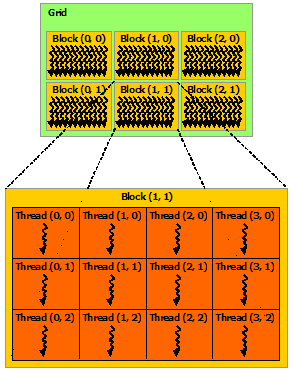
\includegraphics[
				%height=\textheight
				width=1.\columnwidth
				]{fig/thread_hierarchy.png}
		\end{column}
	\end{columns}
\end{frame}
